% !TeX spellcheck = en_US
% !TeX root = ../build/zkevm-network.tex
% !TeX TXS-program:compile = txs:///xelatex/[--shell-escape]



%%%%%%%%%%%%%%%%%%%%%%%%%%%%%%%%%%%%%%%%%%%%%%%%%%%%%%%%%%%%%%%%%%%%%%%%%%
\section{Introduction}

In this section, we will address the interaction of a user with the Polygon zkEVM network through a component known as zkEVM \textbf{JSON-RPC}. To begin, we need to provide an overview of how blocks are generated in L2. We will also provide a detailed explanation of how transactions are processed when they are sent through JSON-RPC, including the validations that occur before they are stored in the \textbf{Pool}. The main components involved in this process are the \textbf{JSON-RPC}, \textbf{Pool}, \textbf{Sequencer}, \textbf{Executor}, Prover \textbf{HashDB}, and Node \textbf{StateDB}.




%%%%%%%%%%%%%%%%%%%%%%%%%%%%%%%%%%%%%%%%%%%%%%%%%%%%%%%%%%%%%%%%%%%%%%%%%%%%%%%%
\section{zkEVM JSON-RPC}

The \href{https://ethereum.org/en/developers/docs/apis/json-rpc}{\textbf{Ethereum JSON-RPC}} is a standardized collection of methods used by all Ethereum nodes, acting as the main interface for users to interact with the network. Figure \ref{fig:eth-json-rpc} illustrates a user querying the Ethereum JSON-RPC to retrieve information on the latest forged block. The user's retrieved data includes all information related to the block, including its transactions.

\begin{figure}[H]
\centering
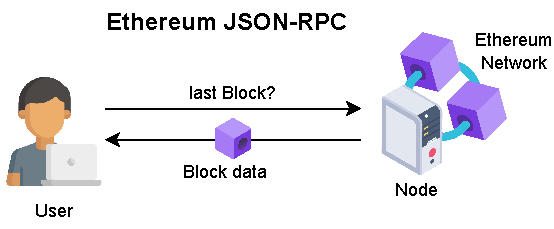
\includegraphics[scale=0.6]{\zkevmdir/figures/architecture/json-rpc/eth-json-rpc.drawio}
\caption{The \textbf{user} asks for information  for the last block and \textbf{Ethereum JSON-RPC} sends it.}
\label{fig:eth-json-rpc}
\end{figure}

For instance, the user can request it as follows:

\begin{lstlisting}[style=termt]
curl -X POST --data '{
  "jsonrpc":"2.0",
  "method":"eth_getBlockByNumber",
  "params":["latest", false],
  "id":1
}' localhost:8545
\end{lstlisting}

The zkEVM architecture refers to \textbf{zkEVM JSON-RPC} as the interface compatible with Ethereum JSON-RPC for any Layer 2 system equal to Ethereum. It replicates the same endpoints and receives similar answers. The zkEVM JSON-RPC incorporates all Ethereum JSON-RPC methods, although some answers from zkEVM JSON-RPC are specifically relevant within the zkEVM context.

The zkEVM JSON-RPC not only includes the methods from the Ethereum JSON-RPC but also offers additional methods to handle zkEVM-specific functionalities. The whole list of available endpoints and their current implementation status can be located in the following link: \href{https://github.com/0xPolygonHermez/zkevm-node/blob/develop/docs/json-rpc-endpoints.md}{json-rpc-endpoints.md}. The API specification for the zkEVM endpoints is available in the \href{https://github.com/0xPolygonHermez/zkevm-node/blob/develop/jsonrpc/endpoints_zkevm.openrpc.json}{endpoints\_zkevm.openrpc.json} file, which follows the OpenRPC standard.

Ethereum's JSON-RPC responds with the most recently created L1 block when requesting the last block. We have batches that transition through various states: \textbf{trusted}, \textbf{virtual}, and \textbf{consolidated}. We will now determine the expected response from the zkEVM JSON-RPC when queried for the latest L2 block.





%%%%%%%%%%%%%%%%%%%%%%%%%%%%%%%%%%%%%%%%%%%%%%%%%%%%%%%%%%%%%%%%%
\section{zkEVM L2 Blocks and Batches}


\subsection{L2 Block Definition}

The primary purpose when defining an L2 block is to minimize delay. We must select between trusted, virtual, or consolidated batches based on this premise. To minimize latency, it is clear that defining trusted batches as L2 blocks is the best choice. The delay in this case is \texttt{close\_a\_batch\_time}, which is the shortest one.

We can keep questioning if the zkEVM can offer a reduced delay. This can be achieved if we generate an L2 block before its associated batch is closed. We can generate L2 blocks that incorporate transactions immediately once their order is determined, meaning once it is established that they will be included in a batch at a specific location. The extreme situation, which is the one that we use in our current design, is that we create an L2 block for each ordered L2 transaction. This minimizes delay by allowing transactions to be processed without waiting for additional transactions to close an L2 block. This delay will be referred to as \texttt{order\_a\_transaction\_time}.


\subsection{Fork-Dragonfruit}

In general, it is important to establish a clear distinction between batches and blocks within the zkEVM framework. An \textbf{L2 batch} represents the minimal data unit for which a proof is generated. On the other hand, an \textbf{L2 block} is the data structure returned to users through the RPC, and it belongs to L2 batches. L2 blocks, as their associated batches, traverse through all zkEVM states: trusted, virtual, and consolidated. From the user's perspective, the block is the visible entity. Up to the fork-dragonfruit (fork-5) included, each L2 block encapsulates a single transaction, adopting the same approach as Optimism. Consequently, every batch contains as many blocks as transactions, it is illustrated in the provided Figure \ref{fig:fork-5}. The formation of a block occurs when the decision is made for the transaction to be included in the trusted state. A \textbf{timestamp} is included as part of part of the batch data, and it is shared across all the blocks within the batch.


\begin{figure}[H]
\centering
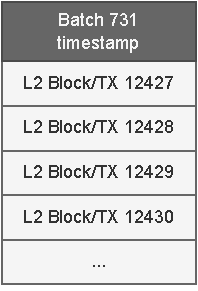
\includegraphics[scale=0.8]{\zkevmdir/figures/architecture/json-rpc/batch-l2-blocks-dragonfruit.drawio}
\caption{A batch with several blocks. Approach fork-dragonfruit (fork-5).}
\label{fig:fork-5}
\end{figure}

\subsection{Fork-Etrog}

Fork-dragonfruit approach assigns each transaction to a block, reducing delay to a minimum that cannot be further decreased beyond \texttt{order\_a\_transaction\_time}. However, this approach has drawbacks as it results in a significant amount of data in the database due to the large number of L2 blocks created. Additionally, it does not offer a method for assigning unique timestamps to each block within a batch, causing issues for Dapps that rely on this parameter to determine the timing of actions performed by smart contracts.

We address these difficulties in the fork-etrog (fork-6), which allows blocks with multiple transactions by implementing a short timeout period when constructing the block to wait for transactions. The sequencer can modify the timestamp of various blocks in a batch by utilizing a specific transaction or marker known as \texttt{changeL2Block}. This transaction is included in the batch to indicate anytime there is a change in blocks and is responsible for modifying the timestamp and the L2 block number. Figure \ref{fig:fork-6} demonstrates the functionality of this new type of transaction.

\begin{figure}[H]
\centering
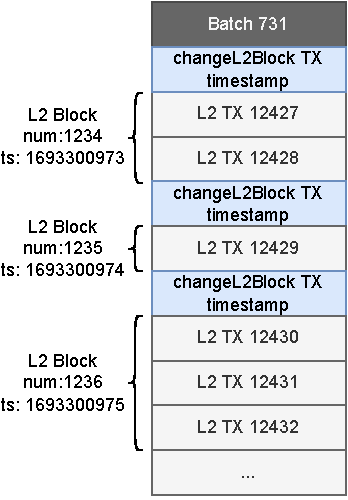
\includegraphics[scale=0.8]{\zkevmdir/figures/architecture/json-rpc/batch-l2-blocks-etrog.drawio}
\caption{Fork-6 new approach including the \texttt{changeL2Block} transaction.}
\label{fig:fork-6}
\end{figure}




%%%%%%%%%%%%%%%%%%%%%%%%%%%%%%%%%%%%%%%%%%%%%%%%%%%%%%%%%%%%%%%%%%%%%%%%%%%%%%%%
\section{Custom zkEVM Endpoints}

%Now we know that when a user queries the JSON-RPC about the last block, the response reflects the most recent L2 block. This L2 block encompasses the latest transactions that have been determined by the trusted sequencer to be ordered within the system. For obtaining this information we use the same RPC call as in Ethereum.
%
%But maybe as a user we don't need the information that our transaction is in a block and we want to know when the batch changes state. For these cases, the zkEVM protocol has extra endpoints to provide extra information about the state of the L2 block. In Figure \ref{fig:isblockvir-req} the user is asking if a block is virtualized using an specific endpoint for it.

When a user requests information from the JSON-RPC regarding the latest block, the response will show the most recent L2 block. This L2 block contains the most recent transactions approved by the trustworthy sequencer to be arranged within the system. We retrieve this information using the identical RPC call as in Ethereum.

Perhaps as users we are not concerned with the status of our transaction being in a block, but rather with when the batch transitions to a new state. The zkEVM protocol has additional endpoints for these circumstances to offer more information regarding the status of the L2 block. For example, the user may ask whether a block is virtualized using a specific endpoint as shown in Figure \ref{fig:is-block-virtualized}.

\begin{figure}[H]
\centering
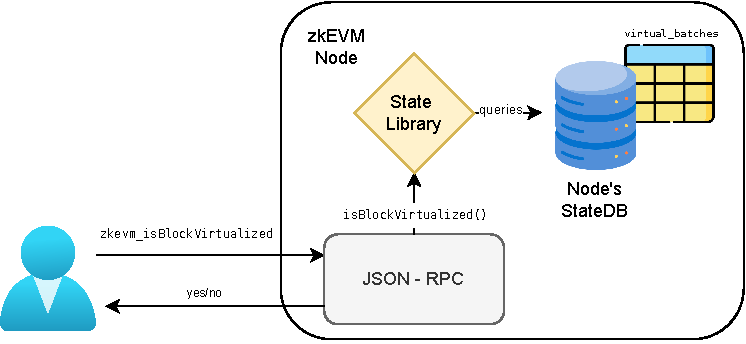
\includegraphics[scale=0.8]{\zkevmdir/figures/architecture/json-rpc/isBlockVirtualized-request.drawio}
\caption{Request from the user for knowing if the block is virtualized.}
\label{fig:is-block-virtualized}
\end{figure}

Here is a collection of the main custom zkEVM endpoints, each accompanied by a brief description.

\begin{itemize}

\item \texttt{zkevm\_consolidatedBlockNumber}: Returns the latest block number within the last verified batch.

\item \texttt{zkevm\_isBlockVirtualized}: Returns true if the provided block number is in a virtualized batch.

\item \texttt{zkevm\_isBlockConsolidated}: Returns true if the provided block number is in a consolidated batch.

\item \texttt{zkevm\_batchNumber}: Returns the latest batch number.

\item \texttt{zkevm\_virtualBatchNumber}: Returns the latest virtual batch number.

\item \texttt{zkevm\_verifiedBatchNumber}: Returns the latest verified batch number.

\item \texttt{zkevm\_batchNumberByBlockNumber}: Returns the batch number of the batch containing the given block.

\item \texttt{zkevm\_getBatchByNumber}: Gets the info of a batch given its number.

\end{itemize}


%TODO: zkEVM and block explorers




%%%%%%%%%%%%%%%%%%%%%%%%%%%%%%%%%%%%%%%%%%%%%%%%%%%%%%%%%%%%%%%%%%%%%
\section{Sending Raw Transactions}
Figure \ref{fig:sendtrans} illustrates the process when a user invokes the \texttt{eth\_sendRawTransaction} endpoint to submit a transaction to the \textbf{PoolDB}.

\begin{figure}[H]
\centering
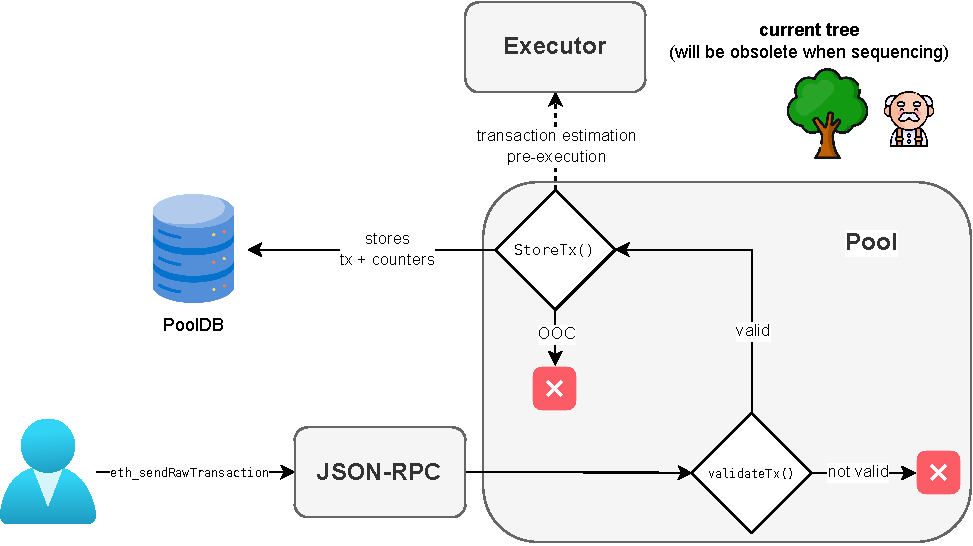
\includegraphics[scale=0.6]{\zkevmdir/figures/architecture/json-rpc/send-raw-transaction.drawio}
\caption{Sending a transaction to the system.}
\label{fig:sendtrans}
\end{figure}

When an L2 transaction is received, \textbf{JSON-RPC} sends it to the \textbf{Pool} component. The \textbf{Pool} component is responsible for, among other things, adding transactions into the \textbf{PoolDB}. The Pool component conducts initial validations on transactions. If any of these validations fail, an error is sent to the JSON-RPC component, which then forwards the error to the user. It also conducts a transaction estimation pre-execution using the current state root, which may differ from the state when the transaction is ultimately ordered.

The first process that takes place in the Pool, as we can see in Figure \ref{fig:sendtrans}, is the \texttt{validateTx()}. In this function take place the preliminary validations:

\begin{enumerate}
\item The transaction IP address has a valid format.

\item The transaction fields are properly signed (in both current and pre-EIP-155). EIP-155 states that we must include the chainID in the hash of the to be signed data (which is an anti replay attack protection).

\item the transaction's \texttt{chainID} is the same as the pool's \texttt{chainID} (which is the \texttt{chainID} of the L2 Network) whenever \texttt{chainID} is not zero.

\item The transaction string has an encoding that is accepted by the zkEVM (more in Section \ref{sec:encoding}). \label{item:encoding}

\item The transaction sender's address can be correctly retrieved from the transaction, using the \href{https://en.wikipedia.org/wiki/Elliptic_Curve_Digital_Signature_Algorithm\#Public_key_recovery}{\textit{ecRecover algorithm}}.

\item The transaction size is not too large (more specifically, larger than 100132 bytes), to prevent DOS attacks.

\item The transaction's value is not negative (which can be the case since we are passing parameters over an API).

\item The transaction sender's address is not present in the \textbf{black list} (that is, is not blocked by the
zkEVM network).

\item The transaction preserves the nonce ordering of the account.

\item The transaction sender account has not exceeded the maximum of transactions to have on the pool per user.

\item The pool is not full (currently, the maximum amount of elements in the queue of pending transactions is 1024).

\item The gas price is not lower than the set \textbf{minimum gas price} (this will be explained in more detail later in a section devoted to \textit{economics}).

\item The transaction sender account has enough funds to cover the costs ($\texttt{value} + \texttt{GasPrice} \cdot \texttt{GasLimit}$).

\item The intrinsic gas of a transaction measures the required gas by the amount of transactional data plus the starting gas for the raw transaction (which is currently of $21000$ or $53000$ in case of being a contract creation transaction). If the provided gas is less than the computed intrinsic gas, the check is not passed.

\item The current transaction gasprice is higher than the other transactions in the \textbf{PoolDB} with the same \texttt{nonce} and \texttt{from}. This is because you cannot replace a transaction with another with less gasprice.

\item The sizes of the transaction's fields are compatible with the \textbf{Executor} needs, more specifically:

\begin{itemize}
	\item \texttt{Data} size: 30000 bytes.
	\item \texttt{GasLimit, GasPrice} and \texttt{Value}: 256 bits.
	\item \texttt{Nonce} and \texttt{chainID}: 64 bits.
	\item \texttt{To}: 160 bits.
\end{itemize}

\end{enumerate}


\subsection{zkEVM Transaction Custom Encoding} \label{sec:encoding}
%TODO: Review

Returning to point \ref{item:encoding} of the \texttt{validateTx()} validations explained before, let's analyze the zkEVM transaction custom encoding. The zkEVM currently only supports \textbf{non-typed transactions}. You can refer to standard transaction encodings in Ethereum for further information. The \texttt{to-be-signed-hash} remains consistent between pre-EIP155 and EIP155 transactions, resulting in identical signatures for these transactions.
\small
\begin{gather*}
\texttt{to-be-signed-hash}_{\texttt{pre-EIP155}} = \texttt{keccak}(\texttt{rlp}(\texttt{nonce}, \texttt{gasPrice}, \texttt{startGas}, \texttt{to}, \texttt{value}, \texttt{data}))\\
\texttt{to-be-signed-hash}_{\texttt{EIP155}} = \texttt{keccak}(\texttt{rlp}(\texttt{nonce}, \texttt{gasPrice}, \texttt{startGas}, \texttt{to}, \texttt{value}, \texttt{data}, \texttt{chainID}, 0, 0))
\end{gather*}
\normalsize

The transaction string used for L2 transactions in the batches is a slightly modified version of the regular transaction string. The goal is to streamline the proving system's processing of L2 transactions.

Let's analyze the handling of a typical EIP155 transaction on our chain with a chain ID of $1101$ and a parity of $1$. We would receive the following transaction string:
\[
\texttt{rlp}(\texttt{nonce}, \texttt{gasPrice}, \texttt{startGas}, \texttt{to}, \texttt{value}, \texttt{data}, \texttt{r}, \texttt{s}, \texttt{v}=2238)
\]

To check the signature, we have to rlp-decode the previous string to extract \texttt{nonce}, \texttt{gaspPrice}, \texttt{startGas}, \texttt{to}, \texttt{value}, \texttt{data}, \texttt{r}, \texttt{s} and \texttt{v}. Then, we have to compute the chain identifier and the parity from the \texttt{v}, in our example:
\begin{gather*}
\texttt{chainID} = \lceil (\texttt{v}-35)/2 \rceil = \lceil (2238-35)/2 \rceil = 1101, \\
\texttt{parity}=\texttt{v}-(2 \cdot \texttt{chainID})-35 = 2238-(2 \cdot 1101)-35 = 1.
\end{gather*}

Then, we have to compute rlp-encoding of the following parameters
\[
\texttt{rlp}(\texttt{nonce}, \texttt{gasPrice}, \texttt{startGas}, \texttt{to}, \texttt{value}, \texttt{data}, 1101, 0, 0),
\]

and compute its Keccak hash:
\[
\texttt{to-be-signed-hash} = \texttt{keccak}(\texttt{rlp}(\texttt{nonce}, \texttt{gasPrice}, \texttt{startGas}, \texttt{to}, \texttt{value}, \texttt{data}, 1101, 0, 0)).
\]

Finally, we have to validate the ECDSA signature over $\texttt{to-be-signed-hash}$ with $\texttt{r}, \texttt{s}$ and the $\texttt{parity}$.

As you may notice, there is a rlp-decoding and a rlp-encoding of the transaction parameters. To just do the decoding once, we can just create the transaction string as the $\texttt{to-be-signed-hash}$ and concatenate the $\texttt{r}$, $\texttt{s}$ and $\texttt{parity}$ which are the only extra parameters required to verify the signature. According to this reasoning, we use the following \textbf{raw transaction string} for the zkEVM L2 transactions:
{
\small
\[
\texttt{rlp}(\texttt{nonce}, \texttt{gasPrice}, \texttt{gasLimit}, \texttt{to}, \texttt{value}, \texttt{data}, \texttt{chainID}, 0, 0) \ | \ \texttt{r} \ | \ \texttt{s} \ | \ \texttt{v} \ | \ \texttt{effectivePercentage}.
\]
}

The $\texttt{parity}$ is expressed in the one-byte $\texttt{v}$ parameter that can take the pre-EIP155 $\texttt{parity}$ values (27 and 28). The parameter \texttt{effectivePercentage} which is a specific parameter of the zkEVM related to the fee system. Since the transaction signature is the same, it is easy to transform standard transactions into our custom format and vice-versa (\href{https://github.com/0xPolygonHermez/zkevm-commonjs/blob/main/src/processor-utils.js}{here} you JS utilities for doing these transformations).


\subsection{Storing Transactions in the \textbf{PoolDB}}

Once the first checks are completed without any errors, the function \texttt{StoreTx()} is executed. The function performs a \textbf{transaction estimation pre-execution}, which involves estimating \textbf{zkCounters} for pricing and prioritization purposes, even if it is based on a potentially incorrect state root. Further details on this will be discussed in another document. An error will be raised and the transaction will not be added to the \textbf{PoolDB} if we get an OCC (out-of-counters) error at this moment.

After the transactions are stored in the \textbf{PoolDB}, the \textbf{Sequencer} chooses certain transactions, attempts to close a batch from them, and then inserts them all into a designated table within the node's \textbf{StateDB}, which monitors the L2 blocks. The \textbf{Sequencer} also updates the \textbf{HashDB} with the L2 state data obtained by pre-executing the batch again. Figure \ref{fig:seq-transactions-pool} illustrates the process. This second batch pre-execution is expected to be correct at this stage of the processing as it uses the current tree to calculate the exact Gas and zkCounters needed.

\begin{figure}[H]
\centering
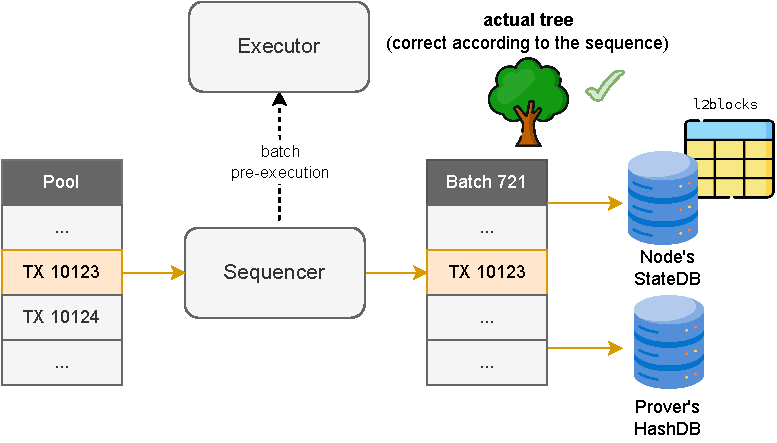
\includegraphics[scale=0.7]{\zkevmdir/figures/architecture/json-rpc/pool-2-trusted-block.drawio}
\caption{A second pre-execution takes place once the Sequencer sequence a certain transaction and includes it in a certain batch. Observe that, in this case, the state root is the correct one. During this second pre-execution, sequencer updates the \textbf{HashDB} accordingly. }
\label{fig:seq-transactions-pool}
\end{figure}

After this process, the \textbf{Executor} performs the last execution known as batch execution during which the \textbf{Prover} can generate the corresponding proof. If all functions correctly, the second pre-execution and the final execution should be identical. The whole process is summarized in Figure \ref{fig:pre-exec-summary}.


\begin{figure}[H]
\centering
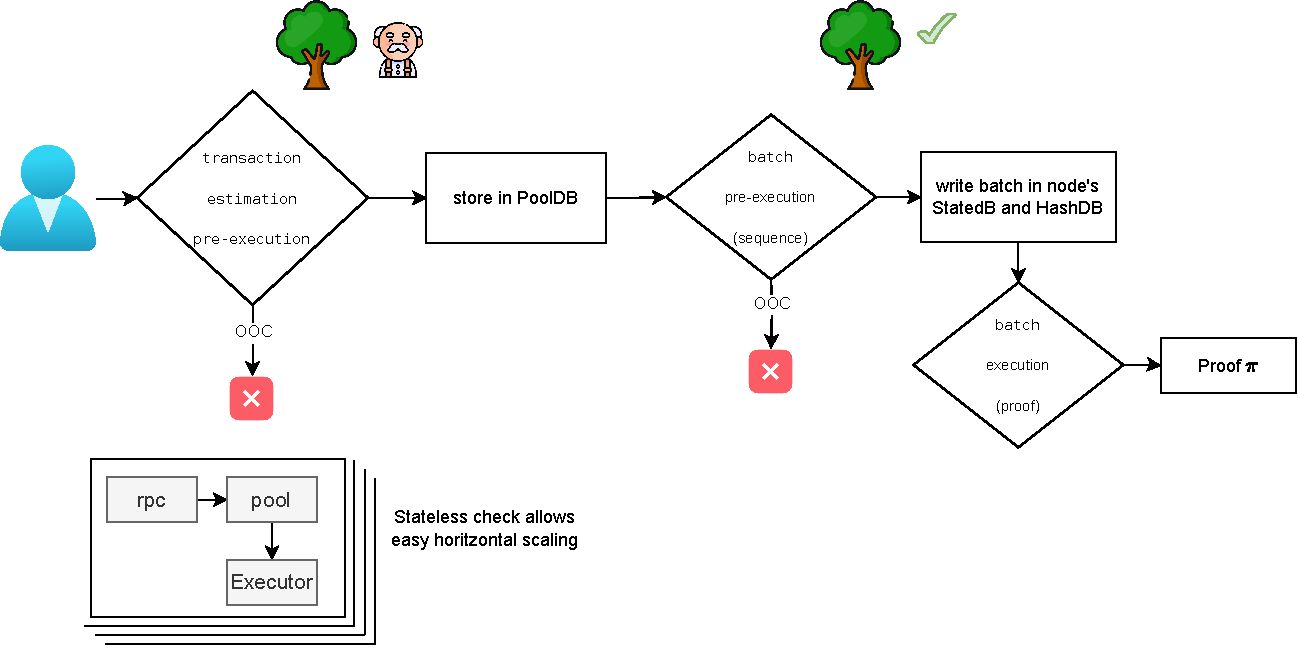
\includegraphics[width=0.8 \textwidth]{\zkevmdir/figures/architecture/json-rpc/pre-executions-summary.drawio}
\caption{Diagram illustrating the three executions occurring between the user sending a transaction and the generation of a proof.}
\label{fig:pre-exec-summary}
\end{figure}

Figure \ref{fig:pre-exec-summary} shows that the counters check is performed twice. The first check is an estimation, while the second one provides the actual values. If all goes as planned, the two final checks should be identical, as previously mentioned.


